\section{模型检验与分析}

为验证本文模型的有效性与稳健性，本节从约束校验、数值收敛、灵敏度与情景稳健性四方面进行检验。

\subsection{约束校验}

对问题一、二、三的每一套最优方案，逐一程序化校验其是否满足全部约束（土地容量、水浇地二季复种、重茬回避、豆类轮作、销售上限），结果见表\ref{tab:validate}。

\begin{table}[htbp]
	\caption{最优方案约束校验结果}
	\label{tab:validate}
	\centering
	\begin{tabular}{ccc}
		\toprule
		方案 & 校验项目数 & 违规数 \\
		\midrule
		问题1 情形1 & 全部约束 & 0 \\
		问题1 情形2 & 全部约束 & 0 \\
		问题2（$\lambda=0.3$） & 全部约束 & 0 \\
		问题3（$\lambda=0.3$） & 全部约束 & 0 \\
		\bottomrule
	\end{tabular}
\end{table}

全部方案的每一地块、每一季次均满足约束，说明模型构建与求解结果在结构上自洽。

\subsection{求解收敛性}

大规模0-1整数规划采用 HiGHS 分支定界求解。以问题1情形1为例，模型含约6800个0-1种植变量、上万个约束，求解约150秒后达到$1\%$相对最优间隙并终止，最优目标值约$3988$万元；情形2在约135秒内收敛到$0.8\%$间隙，最优目标值约$5918$万元。说明解的质量与收敛性满足要求。问题2、3的情景化模型规模更大（$N=30$ 时总变量约1.67万、其中0-1种植变量6762个，约束约2.67万），在$4\%$相对间隙内约数秒至数十秒得到近似最优方案，各情景约束全部满足；因情景数为有限抽样，解的期望收益为下界估计，结论方向稳健。

\subsection{灵敏度分析}

考察目标参数扰动对结果的影响。以问题1情形1方案为基准，在保持种植方案不变的前提下，分别扰动销售单价$r_{c,s}$、亩产量$y_{c,p,s}$、销售量基准$S_{c,s}$与种植成本$c_{c,p,s}$各$\pm5\%$，按题目销售规则重算总收益，观察其变化幅度，结果见表\ref{tab:sensitivity}，龙卷风图见图~\ref{fig:tornado}。

\begin{table}[htbp]
	\caption{参数灵敏度分析结果}
	\label{tab:sensitivity}
	\centering
	\begin{tabular}{cccc}
		\toprule
		参数（$\pm5\%$扰动） & 收益下降 & 收益上升 & 总跨度（万元） \\
		\midrule
		销售单价 $r_{c,s}$ & $-239.6$ & $+239.6$ & $479.2$ \\
		亩产量 $y_{c,p,s}$ & $-203.5$ & $+179.7$ & $383.2$ \\
		销售量基准 $S_{c,s}$ & $-59.9$ & $+36.4$ & $96.3$ \\
		种植成本 $c_{c,p,s}$ & $-29.2$ & $+29.2$ & $58.4$ \\
		\bottomrule
	\end{tabular}
\end{table}

\begin{figure}[htbp]
	\centering
	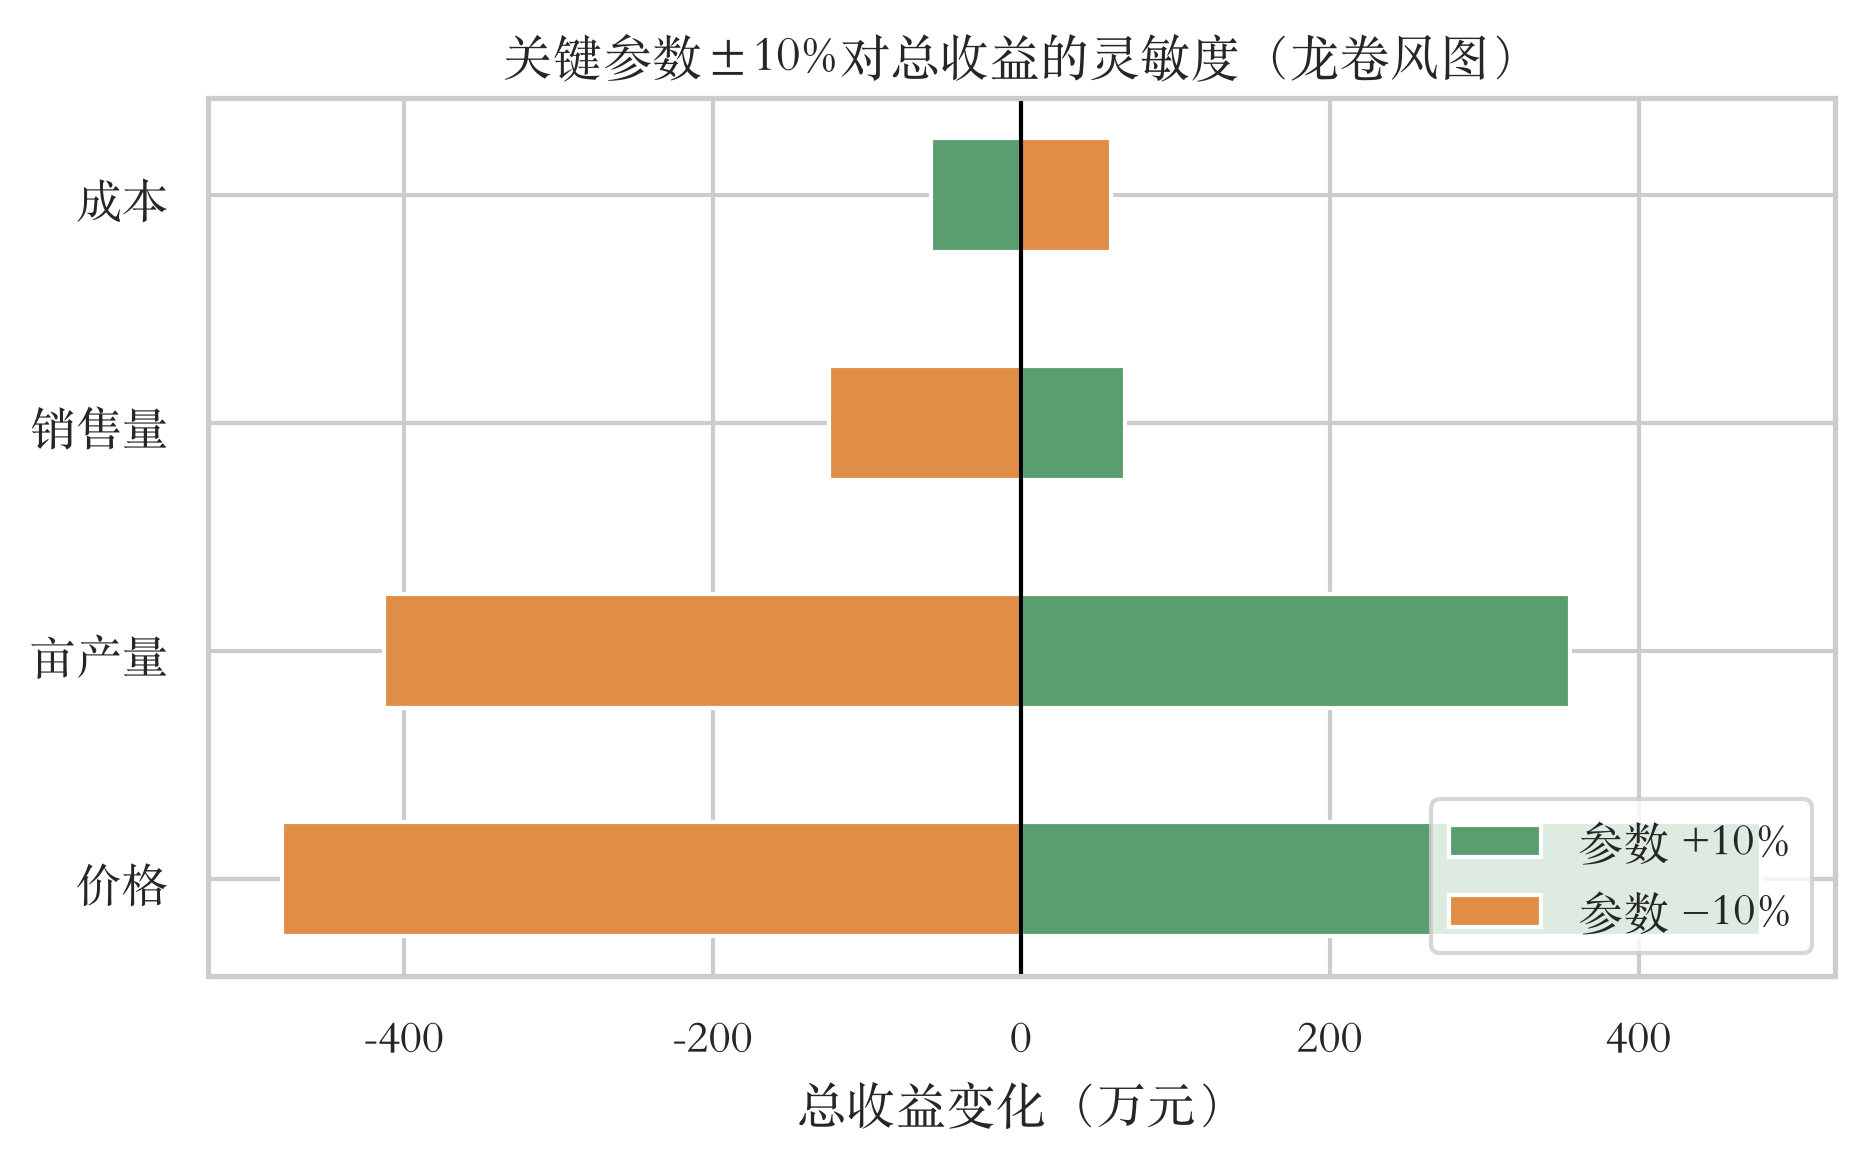
\includegraphics[width=0.62\textwidth]{figures/fig_tornado_q1_1.png}
	\caption{关键参数$\pm10\%$灵敏度龙卷风图}
	\label{fig:tornado}
\end{figure}

可见总收益对销售价格最敏感，其次为亩产量，再次为销售量基准与种植成本。亩产量$\pm5\%$的变化呈明显不对称（$-203.5$万元 vs $+179.7$万元）：产量上升时受销售上限约束，增加的产量无法全部转化为收益，体现了情形1"超产滞销"规则的抑制效应。销售价格主导收益，也解释了问题2、3中蔬菜价格逐年上升对种植结构的牵引作用——收益高的蔬菜类作物种植面积占比随价格上升而提高。

\subsection{情景稳健性}

对问题2、3分别用3组随机种子（问题2：2024、2025、2026；问题3：7、8、9）各生成 $N=30$ 个情景，在 $\lambda=0.3$ 下重复求解，考察方案与风险指标对随机抽样的稳定性，结果见表\ref{tab:seed}。

\begin{table}[htbp]
	\caption{不同随机种子下的风险指标（$N=30$，$\lambda=0.3$）}
	\label{tab:seed}
	\centering
	\begin{tabular}{lccc}
		\toprule
		情景口径（种子） & 期望收益(万元) & 标准差(\%) & CVaR短缺口(万元) \\
		\midrule
		问题2（2024） & 4022.3 & 1.40 & 104.8 \\
		问题2（2025） & 4031.8 & 2.18 & 162.6 \\
		问题2（2026） & 3996.8 & 2.61 & 204.8 \\
		问题3（7） & 4019.3 & 2.46 & 173.8 \\
		问题3（8） & 4013.3 & 2.87 & 220.2 \\
		问题3（9） & 4014.9 & 2.75 & 193.5 \\
		\bottomrule
	\end{tabular}
\end{table}

可见：三组种子下期望收益均稳定在 $4\,000$ 万元附近（问题2为 $3\,996.8\sim4\,031.8$ 万元、问题3为 $4\,013.3\sim4\,019.3$ 万元，波动均在 $1\%$ 以内），说明 $N=30$ 个情景已能较好估计期望收益；三组种子下问题3的收益标准差均高于问题2（$2.46\%\sim2.87\%$ vs $1.40\%\sim2.61\%$），CVaR短缺口的跨种子平均由问题2的 $157$ 万元升至问题3的 $196$ 万元。因此"考虑相关性后组合风险系统性抬升"的结论不依赖于具体抽样，稳健成立。同时，标准差本身存在约 $\pm15\%$ 量级的抽样误差，故本文对风险的定量比较侧重于方向性与倍数级（约 $1.3$--$1.8$ 倍），而非精确点估计。
